\documentclass[tikz,border=10pt]{standalone}
\usepackage[T1]{fontenc}
\usepackage[utf8]{inputenc}
\usepackage{lmodern}
\usepackage{amsmath,amssymb}
\usetikzlibrary{arrows.meta,positioning,shapes.geometric,calc}
\definecolor{jac}{HTML}{73539E}
\definecolor{ink}{HTML}{354052}
\tikzset{
 >=Stealth,
 state/.style={draw=jac,fill=jac!7,rounded corners=5pt,align=center,minimum width=26mm,minimum height=11mm,inner sep=5pt,font=\small},
 action/.style={state,fill=white},
 decision/.style={draw=jac,fill=jac!7,diamond,aspect=2.4,inner sep=1.8pt,align=center,font=\small},
 success/.style={state,draw=teal!75!black,fill=teal!7},
 failure/.style={state,draw=red!70!black,fill=red!5},
 arrow/.style={->,thick,draw=ink},
 note/.style={align=left,font=\footnotesize,text=ink}
}
\begin{document}

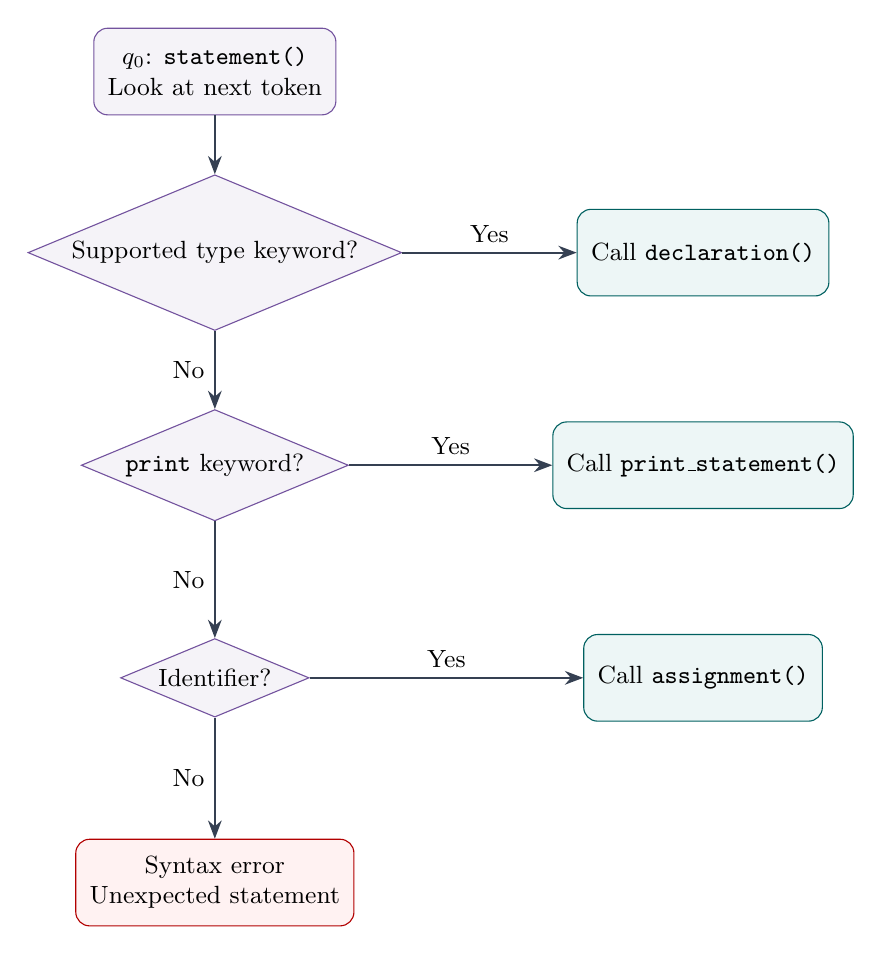
\begin{tikzpicture}[font=\small]
\node[state] (q0) at (0,0) {$q_0$: \texttt{statement()}\\Look at next token};
\node[decision] (d1) at (0,-2.3) {Supported type keyword?};
\node[decision] (d2) at (0,-5) {\texttt{print} keyword?};
\node[decision] (d3) at (0,-7.7) {Identifier?};
\node[success] (decl) at (6.2,-2.3) {Call \texttt{declaration()}};
\node[success] (print) at (6.2,-5) {Call \texttt{print\_statement()}};
\node[success] (assign) at (6.2,-7.7) {Call \texttt{assignment()}};
\node[failure] (bad) at (0,-10.3) {Syntax error\\Unexpected statement};
\draw[arrow] (q0)--(d1);
\draw[arrow] (d1)--node[above]{Yes}(decl);
\draw[arrow] (d1)--node[left]{No}(d2);
\draw[arrow] (d2)--node[above]{Yes}(print);
\draw[arrow] (d2)--node[left]{No}(d3);
\draw[arrow] (d3)--node[above]{Yes}(assign);
\draw[arrow] (d3)--node[left]{No}(bad);
\end{tikzpicture}

\end{document}
